\documentclass[10pt,twocolumn,letterpaper]{article}
\usepackage[pagenumbers]{cvpr}
\usepackage{graphicx,amsmath,amssymb,booktabs,tabularx,listings,xcolor,tikz}
\usetikzlibrary{arrows.meta,positioning}
\usepackage[breaklinks,colorlinks,allcolors=blue]{hyperref}
\usepackage{url}
% Replace every bracketed field before submitting. Add/remove members as needed.
\newcommand{\TeamAuthors}{[Member 1 name, roll number] \\ {}[Member 2 name, roll number] \\ {}[Additional members, if applicable]}
\newcommand{\CourseName}{[Course code and name]}
\newcommand{\FinalRepo}{[INSERT FINAL REVISED GITHUB REPOSITORY URL AND COMMIT]}
\newcommand{\MemberOneContribution}{[Member 1: actual implementation, experiments, writing and presentation contributions]}
\newcommand{\MemberTwoContribution}{[Member 2: actual implementation, experiments, writing and presentation contributions]}
\newcommand{\SubmittingMember}{[Name and roll number of the member submitting this copy]}
\newcommand{\PersonalContribution}{[Specific work completed by the submitting member, with file names or experiment evidence]}

\def\confName{Course Project}\def\confYear{2026}\def\paperID{}
\lstset{basicstyle=\ttfamily\scriptsize,breaklines=true,breakatwhitespace=false,columns=fullflexible,keepspaces=true,showstringspaces=false,numbers=left,numberstyle=\tiny,numbersep=8pt,frame=single,rulecolor=\color{gray!30},tabsize=4}
\title{iMouse: Calibrated Facial Gestures and Adaptive Cursor Control with a Webcam}
\author{\TeamAuthors\\Indian Institute of Technology Kanpur\\\CourseName}
\begin{document}
\maketitle
\begin{abstract}
Hands-free desktop interaction with a standard webcam requires stable pointer movement and separation of intentional gestures from ordinary blinks. We extend an existing OpenCV--MediaPipe--PyAutoGUI controller with neutral calibration, normalized eyelid geometry, a temporal gesture state machine, gesture-aware pointer holds, and speed-adaptive filtering. The design retains the pretrained landmark detector and adds a latest-frame capture path and configurable removal of the mouse library's post-call pause. Its contribution is a task-specific integration and evaluation of established techniques, rather than a new landmark or gaze-estimation algorithm. Supplied offline validation reports a median read-complete-to-dispatch time of 5.33 ms on a repeated-image fixture. Reproduced synthetic tests generate no clicks during 100 bilateral blinks, one click for each of 60 deliberate winks, and reduce stationary coordinate standard deviation from 2.90 to 1.01 pixels. All 33 supplied regression tests pass in a fresh check. These results establish software behavior under controlled inputs; they do not establish live-user accuracy, clinical accessibility, or end-to-end webcam latency.
\end{abstract}

\section{Introduction}
A physical mouse assumes that a user can continuously position and click a handheld device. A webcam interface offers an alternative input channel for hands-busy interaction and motivates exploratory accessibility work. However, tracking a facial landmark is only the first part of an interface. Natural blinks can resemble intentional clicks, small landmark fluctuations can shake the pointer, and serial processing or library sleeps can delay feedback. A useful controller must coordinate these competing actions and communicate its state.

The starting project maps an eye landmark to screen coordinates and uses facial gestures for mouse commands. We retain this lightweight architecture, with no additional model training, and address its control-layer weaknesses. We call the result a \emph{head-assisted iris-position controller}: the pointer depends on iris position in the camera image, which also changes when the head moves. It does not estimate the point of gaze on a display. This distinction agrees with the limitations of MediaPipe Iris~\cite{iris}.

\paragraph{Contribution and novelty.} The course-project contribution is the integration of person-specific neutral calibration, bilateral-blink cancellation, release-confirmed wink clicks, and cursor freezing into a single control policy, combined with adaptive smoothing and explicit latency instrumentation. EAR and One Euro filtering are prior methods~\cite{ear,euro}. We claim an engineering extension of the supplied baseline, not global algorithmic novelty. The evidence supports deterministic gesture handling and synthetic stabilization; a matched human baseline comparison remains necessary to quantify practical benefit.

\section{Related Work and Design Rationale}
\paragraph{Landmark-based perception.} MediaPipe Face Mesh provides facial landmarks, while refined eye landmarks enable iris-position features~\cite{mesh,iris}. We reuse its pretrained inference rather than collect a training dataset or train a new vision model. This lowers implementation effort but inherits the detector's sensitivity to visibility and image quality.

\paragraph{Eye opening and blink detection.} Soukupova and Cech summarize eyelid geometry using the eye aspect ratio and use a temporal classifier for blink detection~\cite{ear}. Our code uses the same geometric idea with calibrated thresholds and explicit temporal rules. It does not reproduce their SVM or claim their dataset results. The controller's task is to reject bilateral blinks and emit a desktop click after a deliberate unilateral wink.

\paragraph{Filtering noisy input.} Casiez et al.'s One Euro filter changes its low-pass cutoff with input speed~\cite{euro}. We use this established method to balance stationary jitter and movement responsiveness. A fixed moving average would also smooth noise but adds a fixed-window delay; adaptive filtering provides explicit controls for the speed/noise trade-off.

\paragraph{Desktop integration.} PyAutoGUI documents a default 0.1-second pause after calls and a corner fail-safe~\cite{pyauto}. The revision makes this pause configurable, defaults it to zero, and retains the fail-safe. OpenCV handles image acquisition~\cite{opencv}. A bounded application-side frame slot prioritizes recent observations, although camera-driver buffering remains outside this guarantee.

\begin{table}[t]
\centering\small
\begin{tabularx}{\columnwidth}{@{}p{.25\columnwidth}XX@{}}
\toprule Component & Supplied baseline & Revised controller\\\midrule
Pointer input & Iris boundary 477 & Mean centers 468, 473\\
Click features & Fixed eyelid gaps & Calibrated EAR\\
Click decision & Per-eye triggers & Wink release; blink cancellation\\
Pointer stability & Direct mapping & Neutral gain + One Euro\\
Scroll & 300-unit bursts & 3-step rate-limited roll\\
Capture & Serial read & Latest-frame webcam slot\\
Mouth action & Exit & Sustained pause/resume\\
Measurement & Trigger counters & Stage timings + tests\\\bottomrule
\end{tabularx}
\caption{Code-level comparison. These are implementation differences, not measured human performance gains.}
\label{tab:comparison}
\end{table}

\section{Problem Definition}
The input is a single RGB webcam stream containing one visible face. The output comprises primary-display cursor coordinates, left/right clicks, vertical scrolling, and a pause/resume state. The default request is $640\times480$ at 30 FPS; actual webcam properties depend on hardware and driver. The interface assumes adequate eye visibility, a stable camera, a roughly frontal pose, and voluntary control of the required gestures. Users who cannot wink independently may need an alternative click mechanism. No depth camera or training stage is required by this implementation.

\section{Proposed Method}
Figure~\ref{fig:overview} summarizes the controller. Perception supplies features; a state machine decides whether an action is permitted before pointer mapping and filtering.
\begin{figure*}[t]
\centering
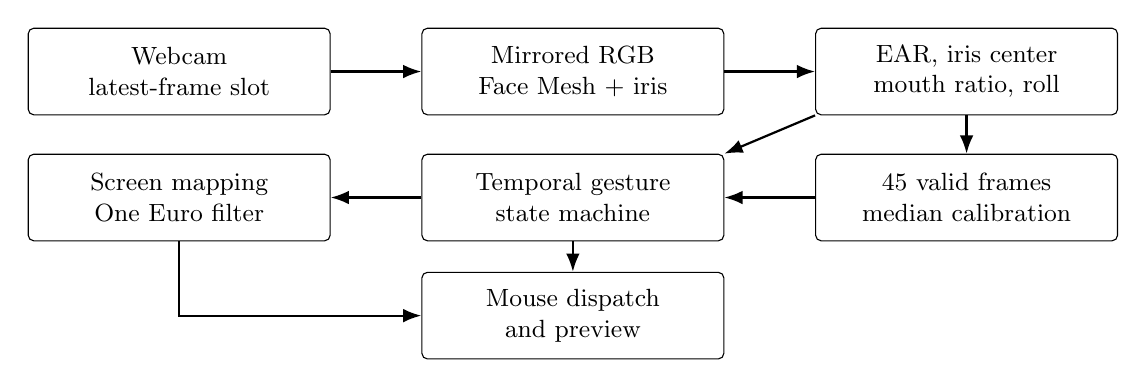
\begin{tikzpicture}[box/.style={draw,rounded corners=2pt,align=center,font=\small,text width=36mm,minimum height=11mm},a/.style={-{Latex},thick}]
\node[box] (cam) at (0,0) {Webcam\\latest-frame slot};
\node[box] (mesh) at (5,0) {Mirrored RGB\\Face Mesh + iris};
\node[box] (feat) at (10,0) {EAR, iris center\\mouth ratio, roll};
\node[box] (cal) at (10,-1.6) {45 valid frames\\median calibration};
\node[box] (gate) at (5,-1.6) {Temporal gesture\\state machine};
\node[box] (map) at (0,-1.6) {Screen mapping\\One Euro filter};
\node[box] (out) at (5,-3.1) {Mouse dispatch\\and preview};
\draw[a] (cam)--(mesh);\draw[a] (mesh)--(feat);\draw[a] (feat)--(cal);
\draw[a] (cal)--(gate);\draw[a] (feat.south west)--(gate.north east);
\draw[a] (gate)--(map);\draw[a] (gate)--(out);\draw[a] (map.south) |- (out.west);
\end{tikzpicture}
\caption{Overview. The gesture policy permits pointer movement only in an appropriate open-eye state. Clicks, scrolling and toggling bypass coordinate filtering. Face loss resets gesture tracking and stops movement.}
\label{fig:overview}
\end{figure*}

\subsection{Acquisition and Feature Geometry}
A reader thread stores only the latest webcam frame, sequence number, and read-complete timestamp. The consumer can skip old frames rather than accumulate a processing backlog. File replay remains serial and uses video time for gesture durations. Each frame is resized only if necessary, mirrored, and converted from BGR to RGB. Face Mesh processes one face with refined landmarks and detection/tracking confidence thresholds of 0.6.

For each eye, use corners $p_1,p_4$ and eyelid pairs $(p_2,p_6)$ and $(p_3,p_5)$:
\begin{equation}
E=\frac{\|p_2-p_6\|_2+\|p_3-p_5\|_2}{2\|p_1-p_4\|_2}.
\end{equation}
Distances use pixel coordinates $(xW,yH)$, avoiding distortion from treating normalized horizontal and vertical coordinates as equal units. The implementation uses indices $(33,133;160,144;158,153)$ for one eye and $(362,263;385,380;387,373)$ for the other. These left/right labels preserve the mirrored baseline mapping; \texttt{--swap-winks} swaps the buttons.

The iris feature is the mean of landmarks 468 and 473. Mouth opening is $M=\|p_{13}-p_{14}\|/\|p_{61}-p_{291}\|$. Head roll $\theta$ is the angle of the line joining eye-corner midpoints, computed with $\operatorname{atan2}$. Eye-corner midpoints reduce coupling between eyelid motion and roll. Invalid geometry or missing landmarks yields no features.

\subsection{Neutral Calibration and Mapping}
The application collects 45 consecutive valid samples with both EAR values above 0.12 and mouth ratio below 0.28. Invalid samples clear this collection. Componentwise medians define neutral iris coordinates $(x_0,y_0)$, open-eye values $(E_{L0},E_{R0})$, and roll $\theta_0$. At 30 processed FPS, 45 samples take approximately 1.5 seconds; this is conditional on valid observations. The lower-level calibration helper permits at least 15 samples, while the application uses 45.

For screen size $(S_w,S_h)$ and gains $(g_x,g_y)$:
\begin{align}
u&=[0.5+g_x(x-x_0)](S_w-1),\\
v&=[0.5+g_y(y-y_0)](S_h-1).
\end{align}
Default gains are 4 and 6. Coordinates are clamped two pixels inside the screen boundary before filtering. This mapping provides controllable movement from image displacement, not a calibration between gaze rays and screen targets.

\subsection{Temporal Gesture Policy}
Each eye closes when $E/E_0<0.55$ and reopens when the ratio reaches 0.75. This hysteresis avoids rapid state changes around one threshold. A wink is eligible only after both eyes have been open for 0.12 seconds. Exactly one eye must close for 0.15--1.0 seconds, and a click is emitted on reopening, subject to a 0.35-second cooldown. If both eyes close at any time, the pending wink is cancelled. The pointer holds while the eyes are closed and during rearming.

Mouth ratio above 0.45 starts a hold. After 0.6 seconds the active state toggles once; a latch prevents repeated toggling while the mouth stays open. A ratio at or below 0.28 releases the mouth state. Normal motion remains blocked until the mouth closes. Thus the toggle occurs at the hold threshold, not at mouth release.

Head roll relative to neutral enters scrolling beyond $12^\circ$ and exits at $7^\circ$ or less. After a 0.18-second hold, the controller emits three scroll units at intervals of at least 0.20 seconds. Pointer movement holds during scrolling. Mouth handling takes precedence over eye gestures, and eye closure suppresses scrolling. Face loss or a gap above 0.5 seconds resets gesture state, preventing stale partial gestures from completing later.

\subsection{Adaptive Smoothing}
For each screen coordinate, let $z_t$ be raw input and $\Delta t$ the elapsed time. Compute raw velocity $d_t=(z_t-z_{t-1})/\Delta t$, then low-pass filter it at 1 Hz to obtain $\widehat d_t$. The position cutoff and update are
\begin{align}
f_t&=f_{\min}+\beta|\widehat d_t|,\\
\alpha(f,\Delta t)&=\frac{1}{1+(2\pi f\Delta t)^{-1}},\\
\widehat z_t&=\widehat z_{t-1}+\alpha(f_t,\Delta t)(z_t-\widehat z_{t-1}).
\end{align}
The defaults are $f_{\min}=1.2$ Hz and $\beta=0.007$ for pixel-valued input. Low speed receives stronger smoothing; larger speed raises the cutoff. Filter state resets after tracking interruptions and gesture transitions. This reduces reuse of stale samples but may produce a position jump on re-entry, which requires live testing.

\subsection{Implementation and Interface}
\texttt{imouse/core.py} contains geometry and control, \texttt{capture.py} owns the reader, and \texttt{app.py} handles inference, desktop dispatch, preview, and CSV/JSON logs. The entry point is \texttt{mouse-controller.py}. Dependencies pin MediaPipe 0.10.21, OpenCV-contrib 4.11.0.86, NumPy 1.26.4, and PyAutoGUI 0.9.54. Python 3.11/3.12 is the project's documented environment. The preview shows active/paused/dry-run state, gestures, landmarks, processing FPS, and inference time. Desktop mode starts paused. SPACE toggles, C recalibrates, and Q/ESC exits when the preview has focus. The physical-mouse corner fail-safe remains available. A Tkinter target task provides ten targets of radius 38 pixels in a nominal $1000\times700$ window.

\section{Experiments and Results}
\subsection{Evidence and Reproducibility}
The numerical timing results below come from the supplied \texttt{results/validation\_report.json} and corresponding CSV, not a newly measured webcam session. The logged environment is Python 3.12.14 on Linux x86\_64, MediaPipe 0.10.21 and OpenCV 4.11.0. CPU model is not recorded, limiting cross-machine comparison. For this documentation, all 33 supplied pytest cases were rerun successfully and the deterministic synthetic experiment was reproduced with the same numerical output. Live webcam/desktop operation was not exercised here.

\paragraph{Data used.} No task-specific training or fine-tuning was performed. The offline fixture repeats a public NASA astronaut image distributed by scikit-image~\cite{astronaut}: 90 face frames, 30 blank frames, then 60 face frames, with a small horizontal translation in part of the first segment. The video is $640\times480$ with a 30 FPS time base. Synthetic feature sequences exercise blinks and winks. Neither fixture is a representative human gesture dataset. The image source and hash are preserved in the supplied result JSON.

\subsection{Offline Pipeline Timing}
All 180 fixture frames were processed, with face features on 150 frames. The recorded throughput is 130.14 processed frames/s for unpaced file replay. It is not a webcam FPS claim. No native mouse actions occurred because the run used dry-run dispatch.
\begin{table}[t]\centering\small
\begin{tabular}{lrr}\toprule Stage & Median (ms) & p95 (ms)\\\midrule
Capture wait & 1.212 & 2.681\\
Preprocessing & 0.178 & 0.538\\
Inference & 4.969 & 10.480\\
Control & 0.072 & 0.204\\
Dry-run dispatch & 0.0012 & 0.0020\\
Read-to-dispatch & 5.328 & 11.573\\
Loop & 6.661 & 12.930\\\bottomrule
\end{tabular}
\caption{Supplied offline fixture timings over all frames, including calibration and no-face frames. These exclude real desktop response.}
\label{tab:timing}\end{table}
Read-to-dispatch begins after the camera/file read completes and includes any wait in the application slot. It excludes exposure, driver buffering and display response. Inference dominates the listed measured compute stages. Per-stage percentiles cannot be added to derive a percentile of total latency. True end-to-end response would require an external measurement of physical action and screen response.
\begin{figure}[t]\centering
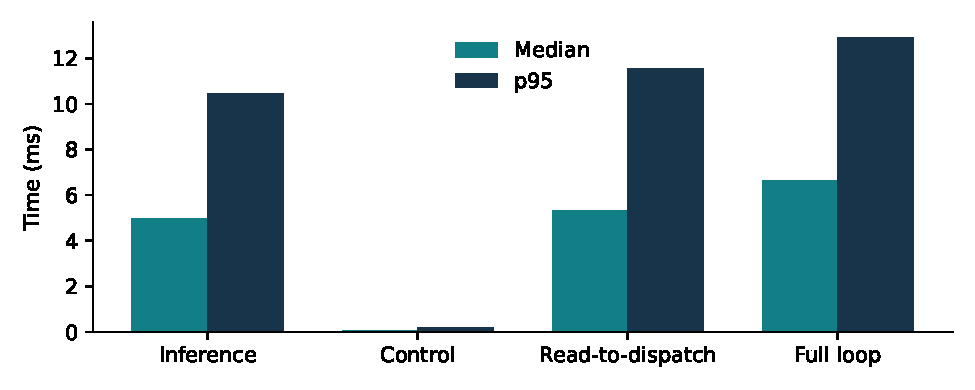
\includegraphics[width=\columnwidth]{figures/timing.pdf}
\caption{Selected supplied timing distributions summarized by median and p95. Dry-run file replay only.}\end{figure}

\subsection{Isolated Library Pause}
The supplied microbenchmark executes PyAutoGUI's installed \texttt{\_handlePause} function for 30 samples at each setting. At 0.1 seconds, the median is 100.128 ms and p95 is 100.205 ms. At zero, these are 0.061 ms and 0.082 ms. This isolates the library sleep; it excludes native mouse calls, perception and display. Removing the pause eliminates an avoidable component but cannot be described as a corresponding speedup of the complete interface. The original PDF's roughly 100--217 ms API-call timings use a different scope and are not a matched baseline comparison.

\subsection{Synthetic Gesture and Jitter Checks}
\begin{table}[t]\centering\small
\begin{tabularx}{\columnwidth}{@{}Xrr@{}}\toprule Scenario & Trials & Emitted clicks\\\midrule
Bilateral blinks & 100 & 0\\
Deliberate left winks & 30 & 30 left\\
Deliberate right winks & 30 & 30 right\\\bottomrule
\end{tabularx}
\caption{Reproduced synthetic-feature checks, including asymmetric onset/release of bilateral blinks. Counts establish these scripted behaviors, not human accuracy.}\end{table}
The generator advances time at 30 Hz and includes asymmetric blink transitions. It directly supplies features, bypassing image detection noise. A separate seed-604 Gaussian coordinate trace contains 300 samples, with a nominal 3-pixel noise scale. Excluding the first 30 samples, standard deviation falls from 2.899 to 1.010 pixels, a 65.2\% reduction computed as $100(1-1.010/2.899)$. The result concerns a stationary synthetic coordinate, not two-dimensional live pointer error or target acquisition speed.
\begin{figure}[t]\centering
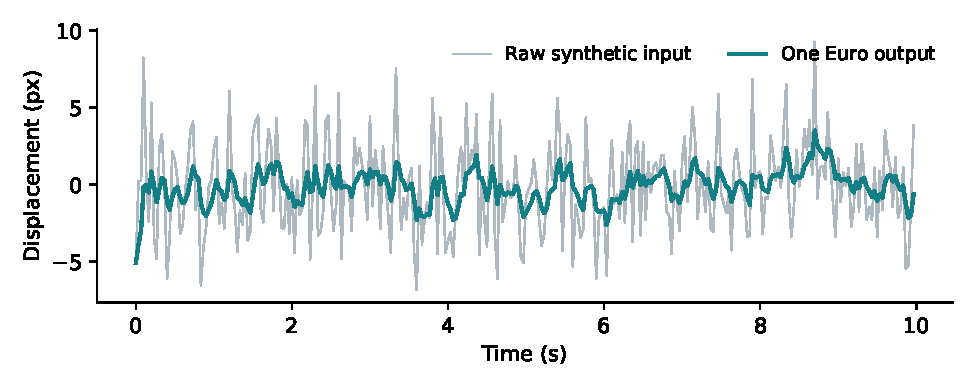
\includegraphics[width=\columnwidth]{figures/jitter.pdf}
\caption{Reproduced stationary noise experiment at 30 Hz. The grey trace is raw input and the teal trace is filtered output. Lower variation does not by itself quantify movement lag.}\end{figure}

\subsection{Required Live Follow-up}
A matched evaluation should alternate original and revised controllers on the same camera, user, lighting, resolution, and target sequence. Log intended actions independently of emitted events. Per participant, a practical protocol includes 20 winks per eye, 30 ordinary blinks, 10 scroll attempts per direction, 10 toggles, and repeated ten-target tasks. Report participants and repetitions explicitly; these are proposed counts, not completed trials.

Useful outcomes are false clicks during ordinary blinks, gesture precision/recall with independently labeled intentions, hit fraction $H/(H+M)$ for targets, and median/p95 acquisition time from target appearance to its first successful hit. Avoid summing the per-miss timestamps: they are cumulative since the same target appeared. Change one mechanism at a time with \texttt{--no-smoothing}, \texttt{--serial-camera}, or \texttt{--mouse-pause 0.1}. Measure live stationary jitter and movement lag together. No live trial values are asserted in this report.

\section{Limitations and Conclusion}
The revision makes the control policy explicit and testable. Software checks support blink cancellation, one click per qualifying wink and noise attenuation, while supplied timing logs identify an avoidable library delay. The design still relies on camera-image displacement, user calibration, and visible facial features. Glasses, dim lighting, rapid movement, inability to wink, and fatigue remain unmeasured. Neutral calibration does not compensate for subsequent large changes in pose or distance. Frame skipping can miss a brief gesture, so latency and recognition must be evaluated together. A control-state overlay and target demo exist, but their usability is unvalidated. Future work should prioritize a consented user comparison and alternative click inputs before adding more gestures or claiming accessibility benefit.

\section*{Individual Contributions and Repository}
\textbf{Submitting member:} \SubmittingMember.\\
\textbf{Specific contribution:} \PersonalContribution.\\
\textbf{Team contributions:} \MemberOneContribution; \MemberTwoContribution. Add all remaining group members before submission.\\
\textbf{Final revised repository:} \FinalRepo.\\
\textbf{Baseline reference:} \url{https://github.com/aksht17/iMouse/tree/c26cb16}. This address is supplied in the project notes and identifies the historical baseline, not proof that the revised code has been published there. The included \texttt{baseline/} script is the inspected comparison source.

\begin{thebibliography}{9}
\bibitem{mesh} Google MediaPipe. Face Mesh documentation and source. \url{https://chuoling.github.io/mediapipe/solutions/face_mesh.html}; \url{https://github.com/google-ai-edge/mediapipe}.
\bibitem{iris} Google MediaPipe. Iris documentation. \url{https://chuoling.github.io/mediapipe/solutions/iris.html}.
\bibitem{ear} T. Soukupova and J. Cech. Real-Time Eye Blink Detection using Facial Landmarks. CVWW, 2016. \url{https://cmp.felk.cvut.cz/ftp/articles/cech/Soukupova-CVWW-2016.pdf}.
\bibitem{euro} G. Casiez, N. Roussel, and D. Vogel. 1 Euro Filter: A Simple Speed-based Low-pass Filter for Noisy Input in Interactive Systems. CHI, 2012, pp. 2527--2530. \url{https://gery.casiez.net/1euro/}; \url{https://github.com/casiez/OneEuroFilter}.
\bibitem{pyauto} A. Sweigart. PyAutoGUI documentation and source. \url{https://pyautogui.readthedocs.io/en/latest/index.html}; \url{https://github.com/asweigart/pyautogui}.
\bibitem{opencv} OpenCV. VideoCapture documentation and source. \url{https://docs.opencv.org/4.x/d8/dfe/classcv_1_1VideoCapture.html}; \url{https://github.com/opencv/opencv}.
\bibitem{astronaut} NASA / scikit-image. Astronaut example image. \url{https://scikit-image.org/docs/stable/api/skimage.data.html#skimage.data.astronaut}; versioned image: \url{https://github.com/scikit-image/scikit-image/blob/v0.24.0/skimage/data/astronaut.png}.
\bibitem{tools} Additional dependency sources. NumPy: \url{https://github.com/numpy/numpy}; JAX: \url{https://github.com/jax-ml/jax}; pytest: \url{https://github.com/pytest-dev/pytest}.
\end{thebibliography}

\clearpage\onecolumn\appendix
\section{Complete Project Code}
The following listings reproduce every Python source file supplied in the project ZIP, including the baseline, application, demo, validation tool and tests. Dependency manifests follow. Third-party dependency source is available through the cited repositories and is not duplicated here. The accompanying source bundle contains raw measurements and documentation. Published revision: \FinalRepo.
\subsection{\texttt{\detokenize{mouse-controller.py}}}
\lstinputlisting[language=Python]{code/mouse-controller.py}

\subsection{\texttt{\detokenize{imouse/__init__.py}}}
\lstinputlisting[language=Python]{code/imouse/__init__.py}

\subsection{\texttt{\detokenize{imouse/core.py}}}
\lstinputlisting[language=Python]{code/imouse/core.py}

\subsection{\texttt{\detokenize{imouse/capture.py}}}
\lstinputlisting[language=Python]{code/imouse/capture.py}

\subsection{\texttt{\detokenize{imouse/app.py}}}
\lstinputlisting[language=Python]{code/imouse/app.py}

\subsection{\texttt{\detokenize{tools/target_practice.py}}}
\lstinputlisting[language=Python]{code/tools/target_practice.py}

\subsection{\texttt{\detokenize{tools/validate_pipeline.py}}}
\lstinputlisting[language=Python]{code/tools/validate_pipeline.py}

\subsection{\texttt{\detokenize{tests/test_core.py}}}
\lstinputlisting[language=Python]{code/tests/test_core.py}

\subsection{\texttt{\detokenize{tests/test_app.py}}}
\lstinputlisting[language=Python]{code/tests/test_app.py}

\subsection{\texttt{\detokenize{baseline/mouse-controller.original.py}}}
\lstinputlisting[language=Python]{code/baseline/mouse-controller.original.py}

\subsection{\texttt{\detokenize{requirements.txt}}}
\lstinputlisting{code/requirements.txt}

\subsection{\texttt{\detokenize{requirements-dev.txt}}}
\lstinputlisting{code/requirements-dev.txt}

\end{document}
